%\documentclass[english]{beamer}
\documentclass[english,hangout]{beamer}
%\documentclass[aspectratio=169]{beamer}
%\usepackage{amsmath}
%\usepackage{amssymb}
\usepackage{rotating}
\usepackage{verbatim}
\usepackage{latexsym}
\usepackage{graphicx}
\usepackage{tabularx}
\usepackage{ragged2e}
\usepackage{eurosym}   % Euro symbol: \euro
\usepackage{listings}
\usepackage{multirow}
\usepackage{colortbl}
\usepackage{textcomp}  % many special symbols
\usepackage{lmodern}
\usepackage{times}
\usepackage[T1]{fontenc}
\usepackage[utf8]{inputenc}
\usepackage[english]{babel}
\usepackage{booktabs}


\usetheme[fb2]{FrankfurtUniversity}
%\usetheme[fb2,noslogan]{FrankfurtUniversity}
%\slogan{\large\color{red}UNAUTHORIZED}


\title{Example Slide Set}
\subtitle{\LaTeX\ beamer theme “FrankfurtUniversity”}
\author{Prof.~Dr.~Eicke Godehardt}
\institute{Frankfurt University of Applied Sciences\\
           Faculty of Computer Science and Engineering\\
           \texttt{godehardt@fb2.fra-uas.de}}
\date{\today}%{January 15, 2015}


\begin{document}


\begin{frame}
\titlepage
\end{frame}
%\addtocounter{framenumber}{-1}


\begin{frame}
\vspace{1.4cm}
\center{\huge\makebox[0pt]{\smash{\fontfamily{ptm}\fontsize{190}{0}\selectfont\color{lightgray}\raisebox{-.5em}[0pt][0pt]{\,'\!'}}}%
If you are not prepared to be wrong, you never come up with anything original.
}

\raggedleft
Sir Ken Robinson
\end{frame}


\begin{frame}
   \frametitle{Agenda}
   \tableofcontents%[hideallsubsections]
\end{frame}



\section{Normal Slide}

\begin{frame}[fragile]
 \frametitle{Example of Normal Slide}
 \framesubtitle{Subtitle}
 Lorem ipsum dolor sit amet, consectetur adipiscing elit. Etiam sit amet
 vulputate ante, vel laoreet erat. Cras pulvinar, sem nec lobortis vehicula,
 leo dolor commodo.
 
  \begin{itemize}
   \item Item 1
   \item Item 2:
     \begin{itemize}
      \item Subitem 2.1
      \item\dots
     \end{itemize}
  \end{itemize}
\end{frame}



\section{Floats}

\subsection{Figures}

\begin{frame}
\frametitle{Figure on slide}
\begin{center}
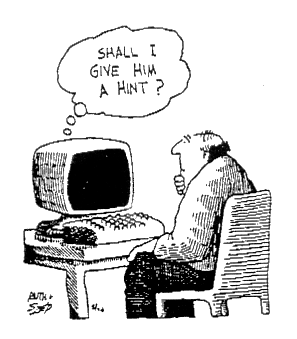
\includegraphics[height=7.5cm]{shall_i_give_him_a_hint.png}
\end{center}
\vspace{-6mm}
\tiny Artist: Tony Auth
\end{frame}



\begin{frame}
\frametitle{Image and Bullet Points Side by Side}
\begin{columns}[onlytextwidth]
\begin{column}{.7\textwidth}
\begin{itemize}
\item \textbf{Lorem ipsum} 
\begin{enumerate}
\item Lorem ipsum dolor sit amet, consectetur adipiscing elit.
\item Donec ut est laoreet, sagittis tortor ac, rhoncus metus.
\end{enumerate}
\item \textbf{Etiam eget} 
\begin{itemize}
\item Etiam eget lectus ac nisl blandit pretium in id velit.
\end{itemize}
\end{itemize}
\end{column}

\begin{column}{.3\textwidth}
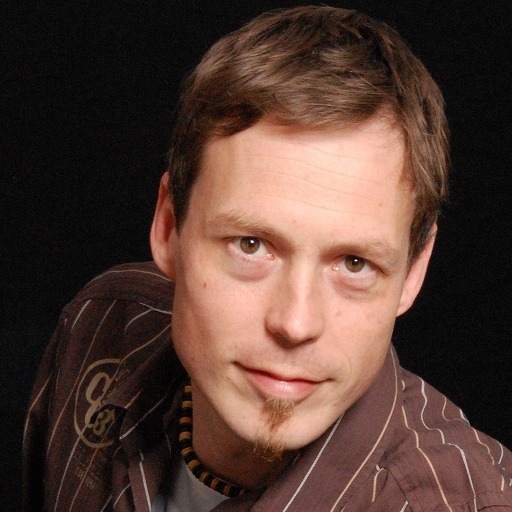
\includegraphics[width=\textwidth]{me}
\end{column}
\end{columns}

\vspace{-.7mm}
\begin{itemize}
\item \textbf{Ut in lorem sollicitudin}
\begin{itemize}
\item Ut in lorem sollicitudin, condimentum magna ac, condimentum urna.
\item Ut malesuada eros id odio rutrum auctor varius a mi.
\item Nulla nec sapien condimentum, faucibus libero at, tristique ante.
\end{itemize}
\end{itemize}
\end{frame}



\subsection{Tables}

\begin{frame}
 \frametitle{Example of a Table}
\begin{table}[ht]
 \begin{tabular}{clrr} \toprule
 2015 (2014)	& 	Language 	& Ratings 	& Change \\
 \midrule
1	(1)		& C		& 16.703\%	& -1.24\% \\
2	   (2)		& Java	& 15.528\%	& -1.00\% \\
3	   (3)		& Objective-C	& 6.953\%	& -4.14\% \\
4	   (4)		& C++	& 6.705\%	& -0.86\% \\
5	   (5)		& C\#		& 5.045\%	& -0.80\% \\
6	   (6)		& PHP	& 3.784\%	& -0.82\% \\
7	   (9)		& JavaScript	& 3.274\%	& \emph{+1.70\%} \\
8	   (8)		& Python	& 2.613\%	& +0.24\% \\
9	 (13)		& Perl	& 2.256\%	& +1.33\% \\
10	 (17)		& PL/SQL	& 2.014\%	& +1.38\% \\
\bottomrule
 \end{tabular}
 \caption{TIOBE Index as of January 2015}
\end{table}
\vspace{-3mm}
\tiny Source: \texttt{http://www.tiobe.com}
\end{frame}



\section{Emphasize}

\subsection{Block}

\begin{frame}
 \frametitle{Using the \texttt{block} environment}
\begin{block}{Title of Bock}
  Content of block goes here.
\end{block}

\begin{exampleblock}{Example No. 42}
  This is an example.
\end{exampleblock}
 
\begin{alertblock}{Watch out!!!}
  You must not do that!
\end{alertblock}
\end{frame}



\subsection{Text Emphasize}

\begin{frame}
 \frametitle{Using the \texttt{\textbackslash emph} command}
You can \emph{emphasize} words by using \texttt{\textbackslash emph\{emphasize\}}.

It will automatically use the color of your faculty.

\vspace{\baselineskip}
BTW you can access all the different colors as \texttt{FB1Color}, \texttt{FB2Color} etc.
\end{frame}



\subsection{Code Blocks}

\begin{frame}[fragile]
 \frametitle{Displaying chunks of code}

\begin{lstlisting}[language=Python]
part = new Part()
part.name = "Sample part"
part.price = 123.45
part.save()
\end{lstlisting}

Another example with \blank{SQL}:

\begin{lstlisting}[language=sql]
INSERT INTO parts (name, price) VALUES ('Sample part', 123.45);
\end{lstlisting}

\begin{alertblock}{You must not forget}
  \dots\ to mark your frame as \texttt{[fragile]}
\end{alertblock}
\end{frame}



\end{document}